\documentclass{article}
\usepackage{listings}
\usepackage{placeins}
\usepackage{siunitx}
\usepackage{graphicx}

\begin{document}
	\begin{titlepage}
		\centering
		\Huge{Experiment 6} \\
		\huge{Characterization of Bipolar Junction Transistors and MOSFETs} \\
		\vspace{1cm}
		\large{EECS 170A - Lab Bench \#1} \\
		\large{\today} \\
		\vspace{1cm}
		\normalsize{Roman Parise (59611417)} \\
		\normalsize{Krishan Solanki (38154673)} \\
		\normalsize{Jason Wang (42873192)} \\
	\end{titlepage}
\section{Procedure}
The objective of this lab is to design a transistor inverter and observe both the switching and amplifier characteristics of MOSFETs. For the first circuit, the switching behavior of a MOSFET is observed. A circuit with multiple components is built and a voltage pulse is given to the transistor to observe the output voltage signal. The input pulse signal is increased so both the turn-on and turn-off transients are observed and the time delay, rise time, and fall time are measured. Next, the circuit for the MOSFET Amplifier is built. The bias voltage is measured without connecting the input source to the amplifier, which should be half of the DC power supply. After measuring, apply an input signal at 10kHz frequency to display both the input and output voltage signal (sinusoidal). The input voltage is increased until the output voltage starts to clamp. The gain is then measured. The upper cutoff frequency is measured along with voltage gain at the certain frequency. Lastly, the cutoff frequency is tested while observing the output after setting the function generator to square wave input. \\

\section{Bipolar Junction Transistor (BJT)}
The BJT is comprised of a linear array of three layers of extrinsic semiconductor materials with alternating types (NPN or PNP). The following figure aids with visualization of the physical structure of the BJT:

\FloatBarrier

\begin{figure}[h!]
	\centering
	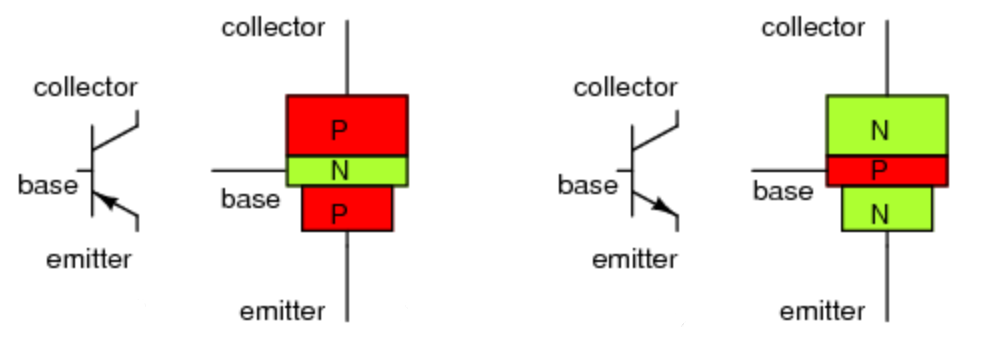
\includegraphics[scale=0.75]{./images/bjt_fig.PNG}
	\caption{Schematic Symbol and Structure of PNP and NPN BJT}
	\label{fig:id_vs_vgs}
\end{figure}

\FloatBarrier

The three layers of semiconductor material form regions called the emitter, base, and collector. The three regions essentially form two semiconductor junctions that share a common thin base region. The emitter region has a significantly higher doping concentration than the other regions. 

Charge generated in the BJT is caused by the diffusion of majority carriers from the emitter to base region. The charge carriers that passed from the emitter to the base are now the excess minority carriers of the region and they diffuse to the collector region due to the thin physical length of the base, which is assumed to be the same order of magnitude of the width of the depletion regions of the semiconductor junctions in the BJT. The thinness of the base layer is crucial so that carriers can diffuse across it much faster than the minority carrier lifetime of the base semiconductor material to prevent loss due to recombination. For a PNP BJT, holes from the p-type emitter diffuse to the n-type base and then diffuse to the p-type collector to generate the collector current across the BJT. For an NPN BJT, electrons from the n-type emitter diffuse to the p-type base and then diffuse to the n-type collector to generate the collector current across the BJT.  In this experiment, an NPN BJT, model MPSA06, is analyzed.

The charge generated by the  NPN BJT is propagated by a forward bias applied across the base-emitter junction ($V_{BE}$) and a reverse bias applied across the base-collector junction ($V_{CE}$). For majority charge carriers (electrons) to overcome the depletion region at the base-emitter junction, a sufficiently large $V_{BE}$ must be applied. At voltage values that are less than that threshold, the carriers cannot overcome the energy barrier at the depletion zone, and therefore the carrier current, $I_C$, is zero. This is referred to as the cut-off region. When the $V_{BE}$ is above the threshold value, the energy barrier is lowered so that the electrons can diffuse from the emitter to base, thus turning on the junction. After the threshold value is met, increase in $V_{BE}$ causes an exponential increase in $I_C$, much like the I-V behavior of a pn-junction diode.

\FloatBarrier

\begin{figure}[h!]
	\centering
	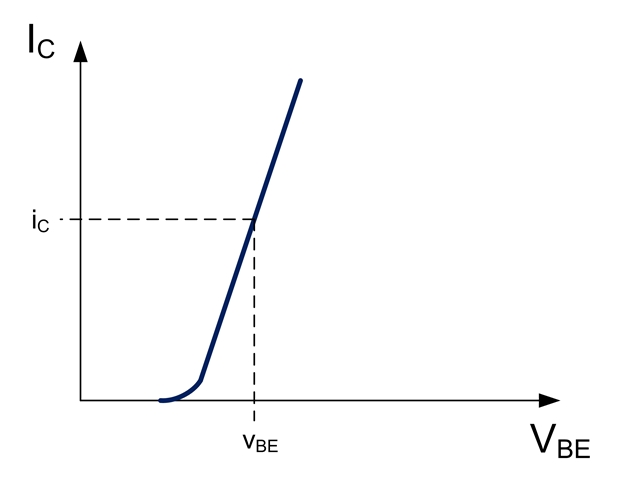
\includegraphics[scale=3]{./images/bjt_ic_vbe_expected.PNG}
	\caption{Expected $I_C$ versus $V_{BE}$ Curve for a NPN BJT}
	\label{fig:ic_vs_vbe}
\end{figure}

\FloatBarrier

After the electrons from the emitter region diffuse to the base region, a sufficiently large voltage must be applied across the base-collector junction for the electrons to then diffuse from the base to the collector region. This voltage is referred to as $V_C$ which is the same as $V_{CE}$ because the emitter in our experimental schematic is grounded. A linear increase in $I_C$ is expected for values of $V_{CE}$ that are less than the amount of voltage in which $V_{BE}$ has overtaken the threshold voltage. As $V_{CE}$ continues to increase, the base region loses so many electrons that the conductivity of the base drops which effectively limits the increase in $I_C$ and $I_C$ is expected to reach a constant maximum beyond that threshold value. The region in which $I_C$ increases linearly is referred to as the saturation region, as the biasing polarity of the collector-base junction is reversed when $V_{CE}$ is lower than the threshold voltage value explained above. Increasing $V_{BE}$ causes $I_C$ to saturate at a larger current value.

\FloatBarrier

\begin{figure}[h!]
	\centering
	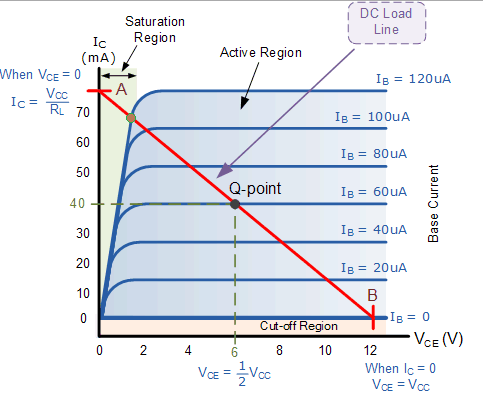
\includegraphics[scale=0.75]{./images/bjt_ic_vce_expected.PNG}
	\caption{Expected $I_C$ versus $V_{E}$ Curve for a NPN BJT}
	\label{fig:ic_vs_vce}
\end{figure}

\FloatBarrier

The following circuit is used to measure and analyze the $I_C - V_{BE}$ and $I_C - V_{CE}$ curves:


\FloatBarrier

\begin{figure}[h!]
	\centering
	\caption{BJT Measurement Circuit}
	\label{fig:bjt_circ}
	\begin{circuitikz}
		\draw
		( 0 , 0 ) node[ npn ] (my_npn) {}
		(my_npn.B) to [ R ] ++( -2 , 0 ) coordinate(r_in)
		(my_npn.B) node[label={ [font=\normalsize] above : $V_{BE}$ } ] { }
		(r_in) to [ battery , v<=$V_1$ ] ++( 0 , -2 ) coordinate(gnd_1)
		(gnd_1) node[ ground ] (my_gnd_1) {}
		(my_npn.E) node[ ground ] (my_gnd_2) {}
		(my_npn.C) to [ R , i<_=$I_C$] ++( 0 , 2 ) coordinate(r_c)
		(my_npn.C) node[label={ [font=\normalsize] below : $V_{CE}$ } ] { }
		(r_c) to [ battery , v<=$V_2$ ] ++( 2 , 0 ) coordinate(gnd_3)
		(gnd_3) node[ ground ] (my_gnd_3) {}
		;
	\end{circuitikz}
\end{figure}

\FloatBarrier

The $I_C - V_{BE}$ plot is measured by fixing $V_2$ at 5V and sweeping $V_1$ from 0V to 5V. $V_{BE}$ is measured by probing the base lead to the emitter lead (ground) of the BJT. The voltage across the resistor connected to the collector lead of the BJT is also probed so that $I_C$ can be calculated from the voltages measured by the probe. $I_C$ has a simple Ohmic relationship with the voltage across the resistor connected to the collector lead. The following values are tabulated following the configuration as described above:

\FloatBarrier

\begin{table}[h!]
	\centering
	\caption{BJT $I_C$ versus $V_{BE}$ Data}
	\label{tab:bjt_ic_vbe}
	\csvautotabular{./tables/bjt_ic_vbe.csv}
\end{table}

\FloatBarrier

{\footnotesize $I_C$ has an Ohmic relationship with the voltage across the resistor connected to the collector, thus $I_C$ is calculated using Ohm's law. The resistor connected to the collector is measured to be 0.998\si{\kilo\ohm} and the resistor connected to the base is 9.902\si{\kilo\ohm}. $V_2$ is fixed to $5$\si{\volt}.}

\FloatBarrier

Subsequently, the following plot is generated from the values in Table \ref{tab:bjt_ic_vbe}:

\begin{figure}[h!]
	\centering
	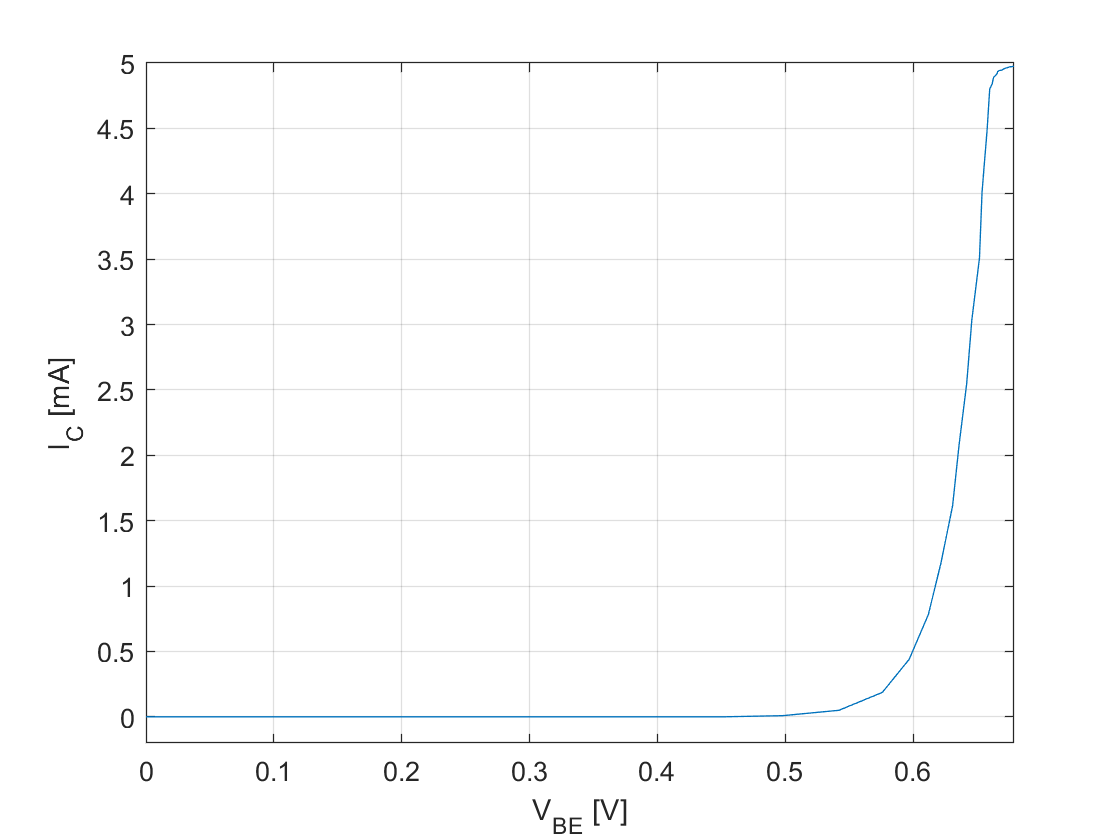
\includegraphics[scale=0.4]{./images/bjt_ic_vbe.PNG}
	\caption{BJT $I_C$ versus $V_{BE}$ Plot}
	\label{fig:bjt_ic_vbe}
\end{figure}

\FloatBarrier

The $I_C - V_{BE}$ curve from the measured values above exhibit the expected behavior. The BJT is observed to turn on when $V_{BE}$ reaches approximately 0.6V. This is consistent with the turn-on voltage of a typical pn-junction diode, which shares its physical composition with the base-emitter junction of the BJT. The curve is then observed to flatten when the $V_{BE}$ becomes closer to $V_{CE}$ as the saturation bias configuration is reached.

The $I_C - V_{CE}$ plot is measured by fixing $V_1$ at 1V and sweeping $V_2$ from 0V to 10V. $V_{CE}$ is measured by probing the collector lead to the emitter lead (ground) of the BJT. The voltage across the resistor connected to the collector lead of the BJT is again probed so that $I_C$ can be calculated from the voltages measured by the probe like before in the previous measuring configuration. The following values are tabulated following the configuration as described above:

\FloatBarrier

\begin{table}[h!]
	\centering
	\caption{BJT $I_C$ versus $V_{CE}$ Data}
	\label{tab:bjt_ic_vce}
	\csvautotabular{./tables/bjt_ic_vce.csv}
	\\
	(\footnotesize $V_1$ is fixed at $1$\si{\volt}.)
\end{table}



\FloatBarrier

Subsequently, the following plot is generated from the values in Table \ref{tab:bjt_ic_vce}:

\FloatBarrier

\begin{figure}[h!]
	\centering
	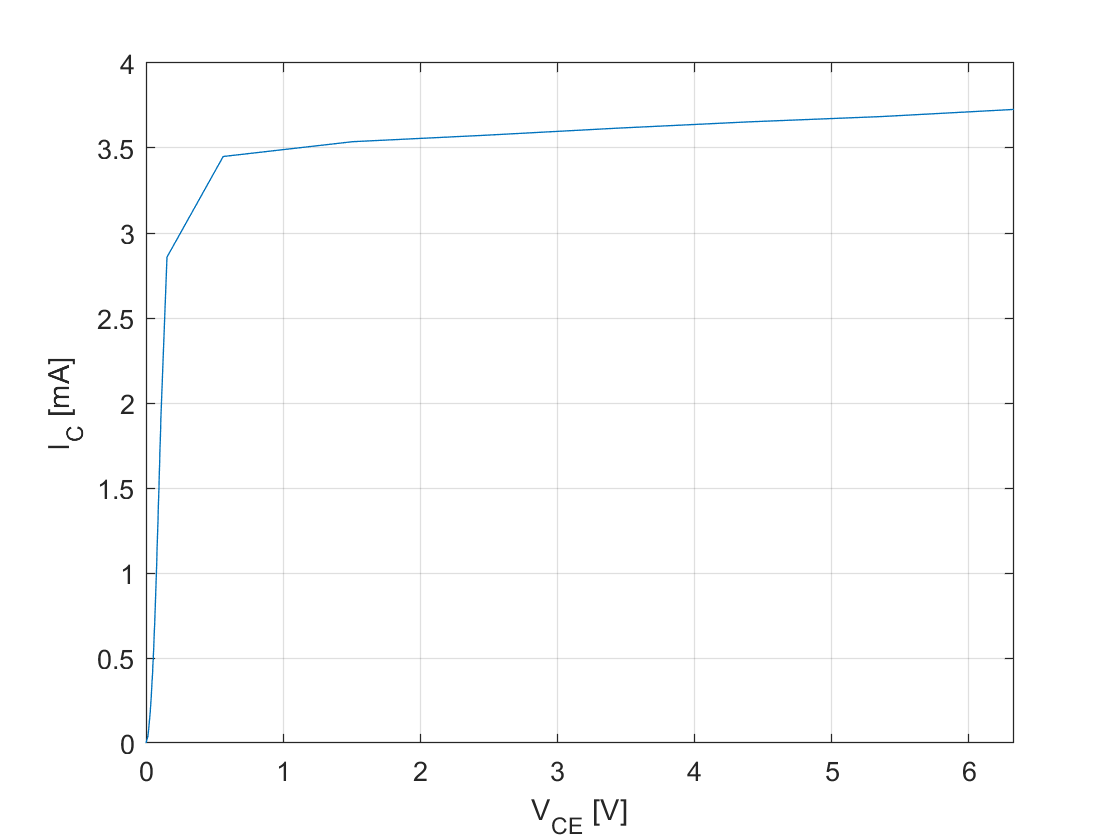
\includegraphics[scale=0.4]{./images/bjt_ic_vce.PNG}
	\caption{BJT $I_C$ versus $V_{CE}$ Plot}
	\label{fig:bjt_ic_vce}
\end{figure}

\FloatBarrier

The $I_C - V_{BE}$ curve from the measured values above again exhibit the expected behavior. The BJT is observed to in the saturation region when $V_{CE}$ is less than approximately 0.6V and $I_C$ is observed to saturate at approximately 3.5mA and the active region is then observed. 

\section{Metal-Oxide Semiconductor Field Effect Transistor}
The source and drain of an n-channel MOSFET are both formed by a metal-semiconductor junction with an n-type region in a p-type substrate. The gate is formed by placing an insulating oxide between a metal contact and the aforementioned p-type substrate. When a high voltage is applied at the gate, this attracts attracts excess electrons toward the gate. The electrons cannot leave the substrate due to the insulating oxide layer. So, they simply build up just below the oxide. The number of electrons in this region, known as the channel, increases considerably. However, by the principle of low-level injection ($\delta p \ll p$ under a perturbation, the applied voltage in this case), the number of holes in the p-type substrate does not change considerably. The conductivity of a semiconductor is given by equation (\ref{eq:cond_semi}):

\begin{equation}
	\label{eq:cond_semi}
	\sigma = q(\mu_n n + \mu_p p)
\end{equation}

Here, $\sigma$ is the conductivity, $q$ is the elementary charge, $\mu_n$ is the electron mobility, $\mu_p$ is the hole mobility, $n$ is the electron concentration, and $p$ is the hole concentration. Since $p$ does not change very much, but $n$ increases considerably, $\sigma$ increases. At a certain point, the channel essentially acts like a conductor. Electrons can now move freely between the source and drain terminals (1).

The situation is actually a bit more complicated. Depletion regions exist between the source and the gate and the gate and the drain. When $V_{GS}$ exceeds a threshold voltage, call it $V_{Th}$, the depletion region is overcome, much like in a pn-junction diode. Since the channel acts as a conductor, electrons, the majority carrier in the source, can now flow freely into the channel between the source and drain terminals. When $V_{GS} \leq V_{Th}$, the diode is "off" and is said to be in the cut-off region. The expected $I_D$ versus $V_{GS}$ plot is shown below. $I_D$ is essentially $0$ in the cut-off region and "turns on" after a certain threshold:

\FloatBarrier

\begin{figure}[h!]
	\centering
	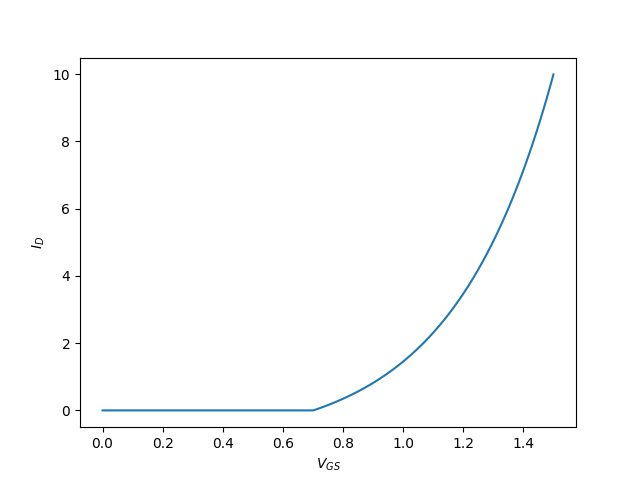
\includegraphics[scale=0.75]{./images/id_vs_vgs.PNG}
	\caption{Expected $I_D$ versus $V_{GS}$ Curve for an n-Channel MOSFET}
	\label{fig:id_vs_vgs}
\end{figure}

\FloatBarrier

Once the electrons have migrated from the source to the channel, the drain-source voltage, or $V_{DS}$ becomes important. Assume the MOSFET is in the "on" state in which $V_{GS} > V_{Th}$. The channel conductance is essentially constant and given by equation (\ref{eq:cond_semi}). Thus, the channel can be modeled as a simple resistor. By increasing $V_{D}$ and therefore $V_{DS}$, the drain can attract electrons more strongly, causing a greater electron current to flow from the drain. So, for small variations in $V_{DS}$, $I_{D}$ increases approximately linearly with $V_{DS}$. This is known as the triode region and occurs when $V_{DS} < V_{GS} - V_{Th}$.

However, this trend cannot continue indefinitely. At a certain point, electrons are so strongly attracted to the drain, that the channel loses many electrons, causing its conductivity to drop. This causes the drain current $I_{D}$ to taper off since the effect of attracting electrons to the drain by increasing $V_{DS}$ is counteracted by the drop in channel conductance. In integrated circuits, the channel width is small enough that the electrons are limited by velocity saturation, causing the same effect (2). This is known as the saturation region and occurs when $V_{GS} - V_{Th} < V_{DS}$ (3). However, with a sufficiently high $V_{DS}$, the voltage may be high enough to produce a strong enough electric field to force electrons from the source through the channel to the drain.

When $V_{GS}$ is increased, a greater electron current flows from the channel to the source. Therefore, the diode can operate in the triode region for longer because it can now draw a larger electron current from the drain to the channel. The saturation region still occurs, but at a higher drain current $I_D$. The expected plot is below with higher values of $V_{GS}$ reaching higher saturation drain currents $I_D$.

% Expected ID vs VDS

\FloatBarrier

\begin{figure}[h!]
	\centering
	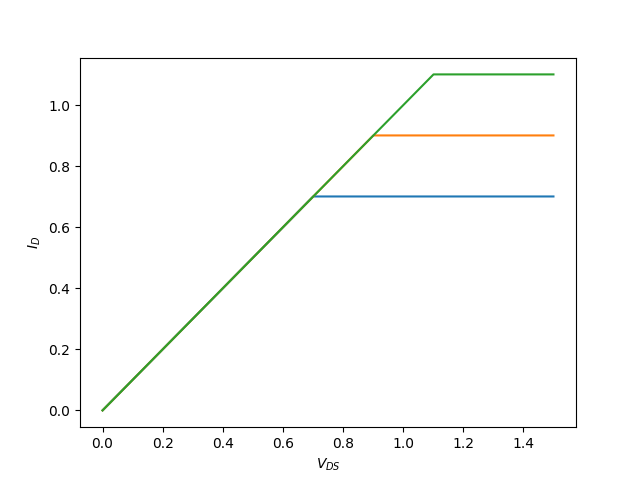
\includegraphics[scale=0.75]{./images/id_vs_vds.PNG}
	\caption{Expected $I_D$ versus $V_{DS}$ Curve for an n-Channel MOSFET}
	\label{fig:id_vs_vds}
\end{figure}

\FloatBarrier

If $V_{DS}$ is held constant and $V_{GS}$ is increased, eventually, $V_{DG}$ drops. If $V_{G}$ becomes sufficiently large relative to $V_{D}$, then the depletion region is not going to be strong enough to actually drive carrier electrons into the drain. So, a larger electron current flows from the channel, but the gate-drain depletion region resists the flow of electrons into the drain. These two effects balance one another out and cause the drain current to level off.

The circuit in figure (\ref{fig:mosfet_circ}) is used to plot the MOSFET curves.

\begin{figure}[h!]
\centering
\caption{MOSFET Measurement Circuit}
\label{fig:mosfet_circ}
\begin{circuitikz}
	\draw
	( 0 , 0 ) node[ nmos ] (my_nmos) {}
	(my_nmos.G) to [ R ] ++( -2 , 0 ) coordinate(r_in)
	(my_nmos.G) node[label={ [font=\normalsize] above : $V_{GS}$ } ] { }
	(r_in) to [ battery , v<=$V_1$ ] ++( 0 , -2 ) coordinate(gnd_1)
	(gnd_1) node[ ground ] (my_gnd_1) {}
	(my_nmos.S) node[ ground ] (my_gnd_2) {}
	(my_nmos.D) to [ R , i<_=$I_D$] ++( 0 , 2 ) coordinate(r_c)
	(my_nmos.D) node[label={ [font=\normalsize] below : $V_{DS}$ } ] { }
	(r_c) to [ battery , v<=$V_2$ ] ++( 2 , 0 ) coordinate(gnd_3)
	(gnd_3) node[ ground ] (my_gnd_3) {}
	;
\end{circuitikz}
\end{figure}

To acquire the $I_D$ versus $V_{GS}$ plot, $V_2$ is fixed at $10$\si{\volt}. $V_1$ is varied to observe different measurement points. It should be noted that because the oxide layer prevents current from flowing from the gate's metal contact to the substrate, no current flows through the gate. Thus, the gate voltage $V_G$ is simply $V_1$. Since the source is grounded, $V_S = 0$, which implies that $V_{GS} = V_G - V_S = V_G = V_1$. Thus, $V_1$ and therefore $V_{GS}$ is varied. As different $I_{D}$ values are observed, the measurements are noted until an $I_{D}$ versus $V_{GS}$ curve is obtained.
Note that gate voltages can be obtained by probing the pins in the MOSFET package. The current $I_D$ can be measured by taking the voltage drop over the resistor connected to the drain and applying Ohm's Law.

\FloatBarrier

\begin{table}[h!]
	\centering
	\caption{MOSFET $I_D$ versus $V_{GS}$ Data}
	\label{tab:mosfet_id_vgs}
	\csvautotabular{./tables/mosfet_id_vgs.csv}
\end{table}

\FloatBarrier

{\footnotesize $I_D$ is acquired by using Ohm's Law with the measured and not the reported resistance values. The resistor connected to the drain is measured to be 0.998\si{\kilo\ohm} and the resistor connected to the gate is 9.902\si{\kilo\ohm}. $V_2$ is fixed to $10$\si{\volt}.}

\FloatBarrier

\FloatBarrier

\begin{figure}[h!]
	\centering
	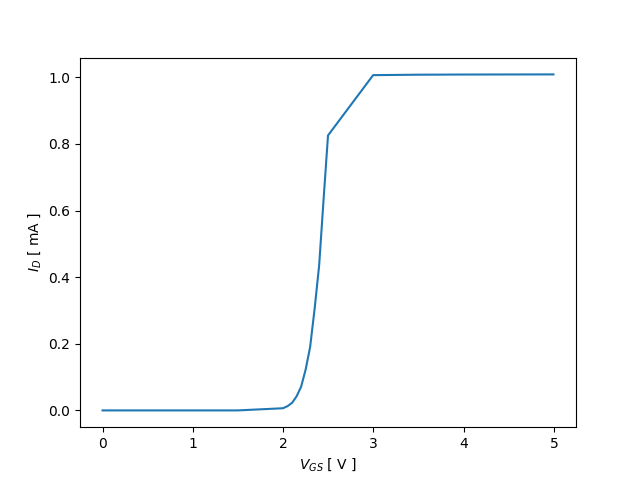
\includegraphics[scale=0.75]{./images/mosfet_id_vgs.PNG}
	\caption{MOSFET $I_D$ versus $V_{GS}$ Plot}
	\label{fig:mosfet_id_vgs}
\end{figure}

\FloatBarrier

The plot in figure (\ref{fig:mosfet_id_vgs}) is precisely as predicted. The MOSFET turns on when $V_{GS}$ exceeds the threshold voltage $V_{Th}$, which is slightly above $2$\si{\volt}. The drain current $I_{D}$ rises exponentially as $V_{GS}$ increases since a larger electron current can now be driven from the channel. Eventually, the curve levels off because the gate voltage $V_{G}$ becomes sufficiently large relative to the drain voltage $V_{D}$, which begins to counteract the flow of electrons into the drain.

To acquire the $I_D$ versus $V_{DS}$ plot, $V_1$ is fixed at about $2.3$\si{\volt}, which is around $V_{Th}$ for the MOSFET as predicted by the previous results. Thus, $V_{GS}$ is fixed. Increasing $V_2$ also increases the drain voltage $V_{D}$ and thus $V_{DS}$ since $V_{DS} = V_D - V_S = V_D$. Again, the drain current $I_D$ can be measured from the voltage over the drain's resistor and Ohm's Law.

\FloatBarrier

\begin{table}[h!]
	\centering
	\caption{MOSFET $I_D$ versus $V_{DS}$ Data}
	\label{tab:mosfet_id_vds}
	\csvautotabular{./tables/mosfet_id_vds.csv}
\end{table}

\FloatBarrier

{\footnotesize $V_1$ is fixed at $2.3$\si{\volt}.}

\FloatBarrier

\FloatBarrier

\begin{figure}[h!]
	\centering
	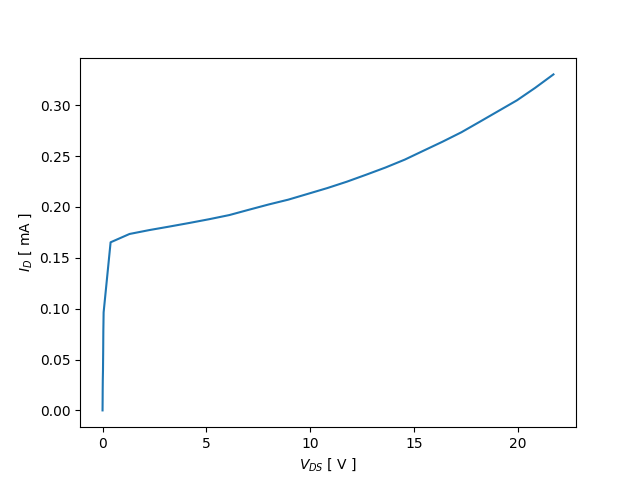
\includegraphics[scale=0.75]{./images/mosfet_id_vds.PNG}
	\caption{MOSFET $I_D$ versus $V_{DS}$ Plot}
	\label{fig:mosfet_id_vds}
\end{figure}

\FloatBarrier

The $I_D$ versus $V_{DS}$ curve is quite close to what is expected. The curve starts off linear when it is in the saturation region. The increased drain voltage relative to the source voltage is similar to increasing the voltage drop over an Ohmic resistor with the channel acting as the resistor. The voltage and current follow a linear relationship. The steepness of the curve reflects the low channel resistance. However, at a certain point, the drain voltage $V_{D}$ becomes very large relative to the gate voltage $V_{G}$. As a result, too many electrons flow to the drain, decreasing the channel's conductance and causing the curve to level off. The growth of the curve at the end is likely due to the very high voltage driving electrons to the drain as described above.

Because $V_1$ is fixed at $2.3$\si{\volt}, $V_{GS} = 2.3$\si{\volt}. The MOSFET operates in the triode region for $V_{DS} < V_{GS} - V_{Th} \approx 2.3$ \si{\volt} $ - 2$ \si{\volt} $ = 0.3$ \si{\volt} assuming $V_{Th} \approx 2$ \si{\volt}. The triode region, though visible, is quite short lived due to the fact that $V_{GS} - V_{Th}$ is only greater than $V_{DS}$ at the very beginning of the curve. As a result, it quickly enters the saturation region. Increasing $V_{GS}$ would prolong the triode region and possibly flatten out the curve afterward.

\section{Discussion}
\subsection{Bipolar Junction Transistor (BJT)}
The $I_C - V_{BE}$ and $I_C - V_{CE}$ curves obtained from experimental measurements are very consistent with theoretically expected behavior for the NPN BJT. The cureves can potentially be smoothened by measuring more intermediate data points at the observed transitions between regions on the curve. This portion of the experiment quantifies the switching behavior of the NPN BJT and it is noted that it is very similar to that of the MOSFET despite fundamental differences in physical structure.
\subsection{Metal-Oxide Semiconductor Field Effect Transistor (MOSFET)}
The $I_D$ versus $V_{GS}$ and $I_D$ versus $V_{DS}$ plots for the n-channel MOSFET are quite accurate to the ones predicted by theory. The only noticeable nonideality occurs when the MOSFET operates in the saturation region an exponential-like increasing curve. This is explained by the fact that $V_{DS}$ becomes high enough to force electrons through the channel. Increasing $V_{GS}$ is a potential way to get a more ideal curve because the linearity of the channel resistance can be maintained if enough electrons are in the channel. The experiment demonstrates the switching behavior of a MOSFET and its similarity to the behavior of a BJT, though the physical specification is different.

\section{Appendix}
The following script is used to generate the expected $I_D$ versus $V_{DS}$ curve for the MOSFET:
\lstinputlisting[breaklines]{./scripts/id_vs_vds.py}
The following script is used to generate the expected $I_D$ versus $V_{GS}$ curve for the MOSFET:
\lstinputlisting[breaklines]{./scripts/id_vs_vgs.py}
The following script is used to generate the tables and figures for the MOSFET:
\lstinputlisting[breaklines]{./scripts/mosfet_data.py}
\section{References}
1. \url{https://coefs.uncc.edu/dlsharer/files/2012/04/J3b.pdf} \\
2. \url{https://inst.eecs.berkeley.edu/~ee40/su05/lectures/lecture13.pdf} \\
3. Lab manual \\
\end{document}
